\documentclass[a4paper]{article}
\usepackage[utf8x]{inputenc}
\usepackage[T1,T2A]{fontenc}
\usepackage[russian]{babel}
\usepackage{hyperref}
\usepackage{indentfirst}
\usepackage{listings}
\usepackage{color}
\usepackage{here}
\usepackage{array}
\usepackage{multirow}
\usepackage{graphicx}
\usepackage{caption}
\graphicspath{{graphics/}}
\usepackage[left=2cm,right=2cm,
top=2cm,bottom=2cm,bindingoffset=0cm]{geometry}
\usepackage{listings}
\lstset{ %
	extendedchars=\true,
	keepspaces=true,
	language=bash,					% choose the language of the code
	basicstyle=\footnotesize,		% the size of the fonts that are used for the code
	numbers=left,					% where to put the line-numbers
	numberstyle=\footnotesize,		% the size of the fonts that are used for the line-numbers
	stepnumber=1,					% the step between two line-numbers. If it is 1 each line will be numbered
	numbersep=5pt,					% how far the line-numbers are from the code
	backgroundcolor=\color{white},	% choose the background color. You must add \usepackage{color}
	showspaces=false				% show spaces adding particular underscores
	showstringspaces=false,			% underline spaces within strings
	showtabs=false,					% show tabs within strings adding particular underscores
	frame=single,           		% adds a frame around the code
	tabsize=2,						% sets default tabsize to 2 spaces
	captionpos=b,					% sets the caption-position to bottom
	breaklines=true,				% sets automatic line breaking
	breakatwhitespace=false,		% sets if automatic breaks should only happen at whitespace
	escapeinside={\%*}{*)},			% if you want to add a comment within your code
	postbreak=\raisebox{0ex}[0ex][0ex]{\ensuremath{\color{red}\hookrightarrow\space}}
}

\begin{document}	% начало документа

\begin{titlepage}	% начало титульной страницы

	\begin{center}		% выравнивание по центру

		\large Санкт-Петербургский Политехнический Университет Петра Великого\\
		\large Институт компьютерных наук и технологий \\
		\large Кафедра компьютерных систем и программных технологий\\[6cm]
		% название института, затем отступ 6см
		
		\huge Телекоммуникационные технологии\\[0.5cm] % название работы, затем отступ 0,5см
		\large Отчет по лабораторной работе №6 \\[0.2cm]
		\large\textbf{"Цифровая модуляция"}\\[5cm]

	\end{center}


	\begin{flushright} % выравнивание по правому краю
		\begin{minipage}{0.25\textwidth} % врезка в половину ширины текста
			\begin{flushleft} % выровнять её содержимое по левому краю

				\large\textbf{Работу выполнила:}\\
				\large Власова А.В.\\
				\large {Группа:} 33501/4\\
				
				\large \textbf{Преподаватель:}\\
				\large Богач Н.В.\

			\end{flushleft}
		\end{minipage}
	\end{flushright}
	
	\vfill % заполнить всё доступное ниже пространство

	\begin{center}
	\large Санкт-Петербург\\
	\large \the\year % вывести дату
	\end{center} % закончить выравнивание по центру

\thispagestyle{empty} % не нумеровать страницу
\end{titlepage} % конец титульной страницы

\vfill % заполнить всё доступное ниже пространство

\section{Цель работы}
 Изучение методов модуляции цифровых сигналов.

\section{Постановка задачи}
\begin{itemize}
	\item Получить сигналы BPSK, PSK, OQPSK, genQAM, MSK, M-FSK модуляторов
	\item Построить их сигнальные созвездия
	\item Провести сравнение изученных методов модуляции цифровых
	сигналов
\end{itemize}


\section{Теоретический раздел}
При цифровой модуляции передаче подлежит не аналоговый модулирующий сигнал, а последовательность целых чисел n0, n1, n2, …, которые могут принимать значения из некоторого фиксированного конечного множества. Эти числа, называемые символами (symbol), поступают от источника информации с периодом T, а частота, соответствующая этому периоду, называется символьной скоростью (symbol rate): fT = 1/T.\\

Последовательность передаваемых символов является дискретным сигналом. Поскольку символы принимают значения из конечного множества, этот сигнал фактически является и квантованным, то есть его можно назвать цифровым сигналом. Типичный подход при осуществлении передачи дискретной последовательности символов состоит в следующем. Каждому из возможных значений символа сопоставляется некоторый набор параметров несущего колебания. Эти параметры поддерживаются постоянными в течение интервала T, то есть до прихода следующего символа.\\

Такой способ модуляции, когда параметры несущего колебания меняются скачкообразно, называется манипуляцией. Существуют следующие типы манипуляций:
\begin{itemize}
	\item амплитудная манипуляция;
	\item фазовая манипуляция;
	\item частотная манипуляция;
	\item квадратурная амплитудная манипуляция.
\end{itemize}

Фазовая манипуляция (PSK) - один из видов фазовой модуляции, при которой фаза несущего колебания меняется скачкообразно в зависимости от информационного сообщения.\\

Двоичная фазовая манипуляция (BPSK) - самая простая форма фазовой манипуляции. Работа схемы двоичной ФМн заключается в смещении фазы несущего колебания на одно из двух значений, нуль или $\pi$  (180°). Двоичную фазовую манипуляцию можно также рассматривать как частный случай квадратурной манипуляции.\\

Квадратурная амплитудная манипуляция (QAM) - манипуляция, при которой изменяется как фаза, так и амплитуда сигнала, что позволяет увеличить количество информации, передаваемой одним состоянием (отсчётом) сигнала.\\

Частотная манипуляция - вид манипуляции, при которой скачкообразно изменяется частота несущего сигнала в зависимости от значений символов информационной последовательности. В случае манипуляции с минимальным сдвигом частоты (MSK), индекс модуляции равен 0,5. Тогда разность частот сигналов, соответствующих различным битам, равна половине скорости передачи информации.

 
\newpage 
\section{Ход работы}
Получим сигналы BPSK, PSK, OQPSK, genQAM и MSK модуляторов и построим их сигнальные созвездия.

\captionof{lstlisting}{Код программы}
\lstinputlisting{../lab6.m}

Полученные сигнальные созвездия представлены на рисунках ниже.

\begin{center}
	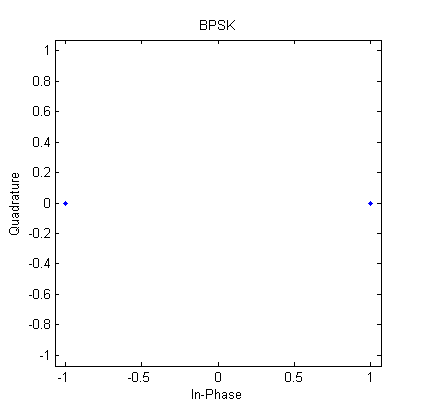
\includegraphics[scale = 1]{bpsk.png} \\Рис.1 Сигнальное созвездие BPSK
\end{center}
\begin{center}
	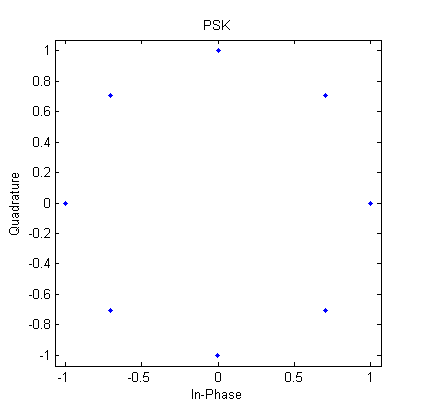
\includegraphics[scale = 1]{psk.png} \\Рис.2 Сигнальное созвездие PSK 
\end{center}
\begin{center}
	\includegraphics[scale = 1]{OQPSK.png} \\Рис.3 Сигнальное созвездие OQPSK
\end{center}
\begin{center}
	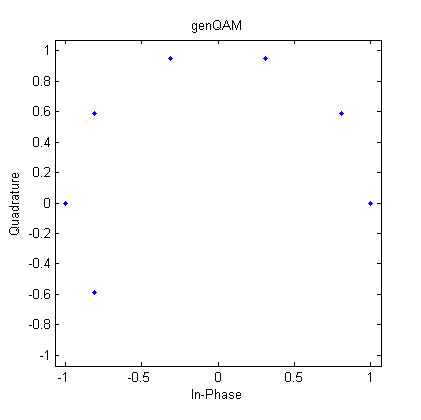
\includegraphics[scale = 1]{genqam.png} \\Рис.4 Сигнальное созвездие genQAM
\end{center}
\begin{center}
	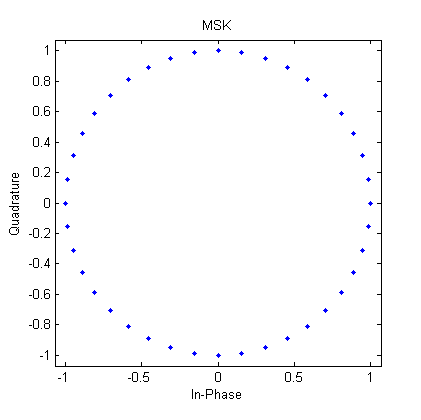
\includegraphics[scale = 1]{msk.png} \\Рис.5 Сигнальное созвездие MSK
\end{center}

\section{Выводы}
В ходе выполнения лабораторной работы получены навыки цифровой модуляции сигналов. Выбор того или иного вида манипуляции обуславливается требованиями к помехозащищенности и пропускной способности канала. Наибольшей помехоустойчивостью обладают те модуляторы, у которых наименьшее число уровней модуляции (количество состояний несущей и скорость передачи). Следовательно, наиболее помехоучтойчивы из рассмотренных модуляторов MSK и BPSK модуляторы. Самую большую пропускную способность имеет QAM модулятор.  
\end{document}



